%----------------------------------------------------------------------------------------
%	PACKAGES AND OTHER DOCUMENT CONFIGURATIONS
%----------------------------------------------------------------------------------------
\PassOptionsToPackage{svgnames}{xcolor}
\documentclass{article}

\usepackage{fancyhdr} % Required for custom headers
\usepackage{lastpage} % Required to determine the last page for the footer
\usepackage{extramarks} % Required for headers and footers
\usepackage{graphicx} % Required to insert images
\usepackage{lipsum} % Used for inserting dummy 'Lorem ipsum' text into the template
\usepackage{amsmath}
\usepackage{mathtools}
\usepackage{float}


\usepackage{listings}
\usepackage{color}

\definecolor{dkgreen}{rgb}{0,0.6,0}
\definecolor{gray}{rgb}{0.5,0.5,0.5}
\definecolor{mauve}{rgb}{0.58,0,0.82}

\lstset{frame=tb,
  language=Java,
  aboveskip=3mm,
  belowskip=3mm,
  showstringspaces=false,
  columns=flexible,
  basicstyle={\small\ttfamily},
  numbers=none,
  numberstyle=\tiny\color{gray},
  keywordstyle=\color{blue},
  commentstyle=\color{dkgreen},
  stringstyle=\color{mauve},
  breaklines=true,
  breakatwhitespace=true,
  tabsize=3
}


% Margins
\topmargin=-0.45in
\evensidemargin=0in
\oddsidemargin=0in
\textwidth=6.5in
\textheight=9.0in
\headsep=0.25in 

\linespread{1.1} % Line spacing

% Set up the header and footer
\pagestyle{fancy}
\lhead{\hmwkAuthorName} % Top left header
\rhead{ \hmwkTitle} % Top right header
\lfoot{\lastxmark} % Bottom left footer
\cfoot{} % Bottom center footer
\rfoot{Page\ \thepage\ of\ \pageref{LastPage}} % Bottom right footer
\renewcommand\headrulewidth{0.4pt} % Size of the header rule
\renewcommand\footrulewidth{0.4pt} % Size of the footer rule

\setlength\parindent{0pt} % Removes all indentation from paragraphs

%----------------------------------------------------------------------------------------
%	DOCUMENT STRUCTURE COMMANDS
%	Skip this unless you know what you're doing
%----------------------------------------------------------------------------------------

% Header and footer for when a page split occurs within a problem environment
\newcommand{\enterProblemHeader}[1]{
\nobreak\extramarks{#1}{#1 continued on next page\ldots}\nobreak
\nobreak\extramarks{#1 (continued)}{#1 continued on next page\ldots}\nobreak
}

% Header and footer for when a page split occurs between problem environments
\newcommand{\exitProblemHeader}[1]{
\nobreak\extramarks{#1 (continued)}{#1 continued on next page\ldots}\nobreak
\nobreak\extramarks{#1}{}\nobreak
}

\setcounter{secnumdepth}{0} % Removes default section numbers

\bibliographystyle{plain}

   
%----------------------------------------------------------------------------------------
%	NAME AND CLASS SECTION
%----------------------------------------------------------------------------------------

\newcommand{\hmwkTitle}{Planning\ Project} % Assignment title
\newcommand{\hmwkDueDate}{Monday,\ Jan\ 09,\ 2017} % Due date
\newcommand{\hmwkClass}{Planning and Scheduling\ } % Course/class
\newcommand{\hmwkClassTime}{09:00am} % Class/lecture time
\newcommand{\hmwkClassInstructor}{Prof. Dr.-Ing. Gerhard K. Kraetzschmar | M.Sc Iman Awaad} % Teacher/lecturer
\newcommand{\hmwkAuthorName}{Chaitanya Hebbal | Mazin Eltayeb | Hashem Talaat} % Your name

%----------------------------------------------------------------------------------------
%	TITLE PAGE
%----------------------------------------------------------------------------------------

\title{
\vspace{2in}
\textmd{\textbf{\hmwkClass\ \\ \hmwkTitle}}\\
%\normalsize\vspace{0.1in}\small{Due\ on\ \hmwkDueDate}\\
\vspace{0.1in}\large{\textit{\hmwkClassInstructor\ }}
\vspace{3in}
}

\author{\textbf{\hmwkAuthorName}}
\date{$9^{th}$ January 2017} % Insert date here if you want it to appear below your name

%----------------------------------------------------------------------------------------

\usepackage{graphicx}
\begin{document}

\maketitle
\newpage

\section{Choosing a planner}

In this project, we started by looking into the results of the 2014 IPC planning competition \cite{ipc}  for the category sequential optimal. The approach was to start at the top of the results list and use the first planner we can compile and run as all planners in the category sequential optimal should be suitable for the given problem.

At first we installed SymBA*-2 \cite{symba2} (After a struggle in compiling the code. Where eventually we had to correct one line of code for a syntax error !!). However, the planner failed during search stage and no plans could be found. Moreover, the planner lacks documentation (and not even a readme file was provided). Therefore, SymBA*-2 was abandoned and we moved into cGamer \cite{cGamer} as SymBA*-1 \cite{symba2} is just an earlier version of SymBA*-2 and suffers from the same problems mentioned above.

In summary, cGamer was the chosen planner as it is the highest performing planner (according to competition results) that we were able to compile, run and use.

\section{Planner Installation \& Challenges}

As expected compiling the planner start with a ton of errors. These errors were fixed by:
\begin{enumerate}
	\item Installing missing package: flex and gcc-multilib.
	\item Editing the cmake files to be compatible with 64 bit processor as instructed in the readme file fo the planner.
	\item Editing the cmake files to use the correct jdk directory.
\end{enumerate}

After successful compilation, the plan was run successfully on the simple domain (with no action costs and no constraints) and was able to produce results for all three problems in the simple domain.

However, when running the planner for with the extended domain that considers action costs (distance), the planner failed to parse the PDDL problem definition files for all three problem. Although, the files are syntactically accurate as it worked with other planners. 

We suspect that the planner supports only a subset of PDDL syntax. For the extended domain we solved using MIPS and METRIC\_FF planners provided as part of the itSimple planning IDE.

\section{Modelling domains and problems}

For modelling the domains and problems, we used itSimple planning IDE \cite{itsimple}. The IDE has uses UML diagrams to model the domains and create problem instances. Following a one hour tutorial, it was straight forward to model the simple domain with no constraints and no actions' costs.

The domain has three object types: robot, object and station. Only robot is an active agent and can : move from one station to another station, pick an object and drop an object. Figure \ref{fig:usecase} below, shows the use case diagram for the all domains.

\begin{figure}[H] %  figure placement: here, top, bottom, or page
	\centering
	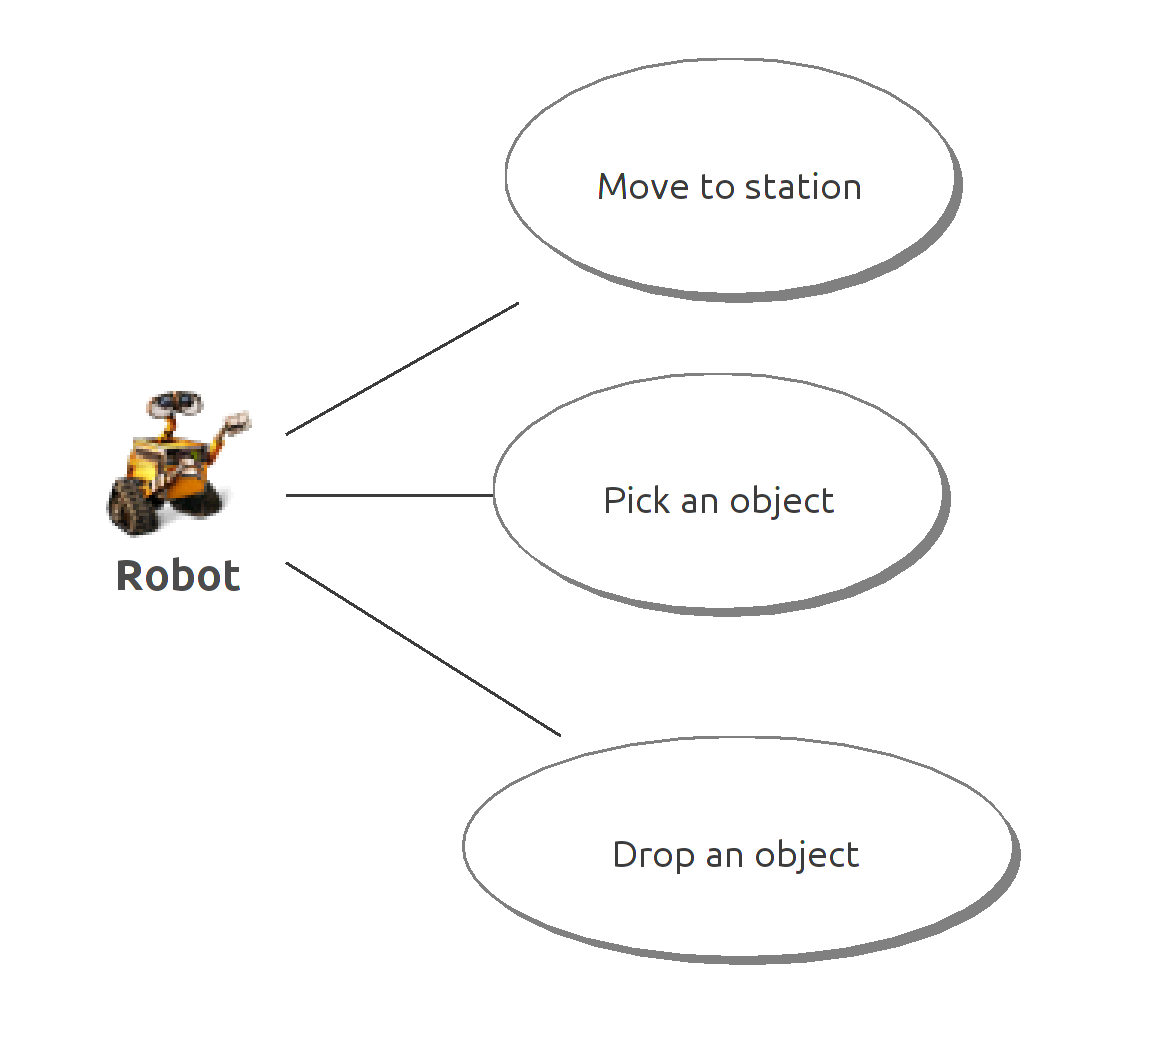
\includegraphics[width=8 cm]{figures/use_case_diagram.png} 
	\caption{Robocup at work domain: Use case diagram}
	\label{fig:usecase}
\end{figure}

To consider distances, the domain was altered by adding a utility function that calculates the distance between two location. A utility attribute was added to keep track of the travelled distance. An effect was added to the move action to increase the total distance by the amount of the distance travelled.

The constraint on the number of objects the robot can carry is implemented by adding two attributes one represent the capacity of the robot and another for the current load. The capacity is fixed at 3. A new precondition for the pick action was added to make sure the current load is less than the capacity. Effects were added to pick action to increase current load and to drop action to decrease current load. Figure \ref{fig:class} shows the final class diagram.

\begin{figure}[H] %  figure placement: here, top, bottom, or page
	\centering
	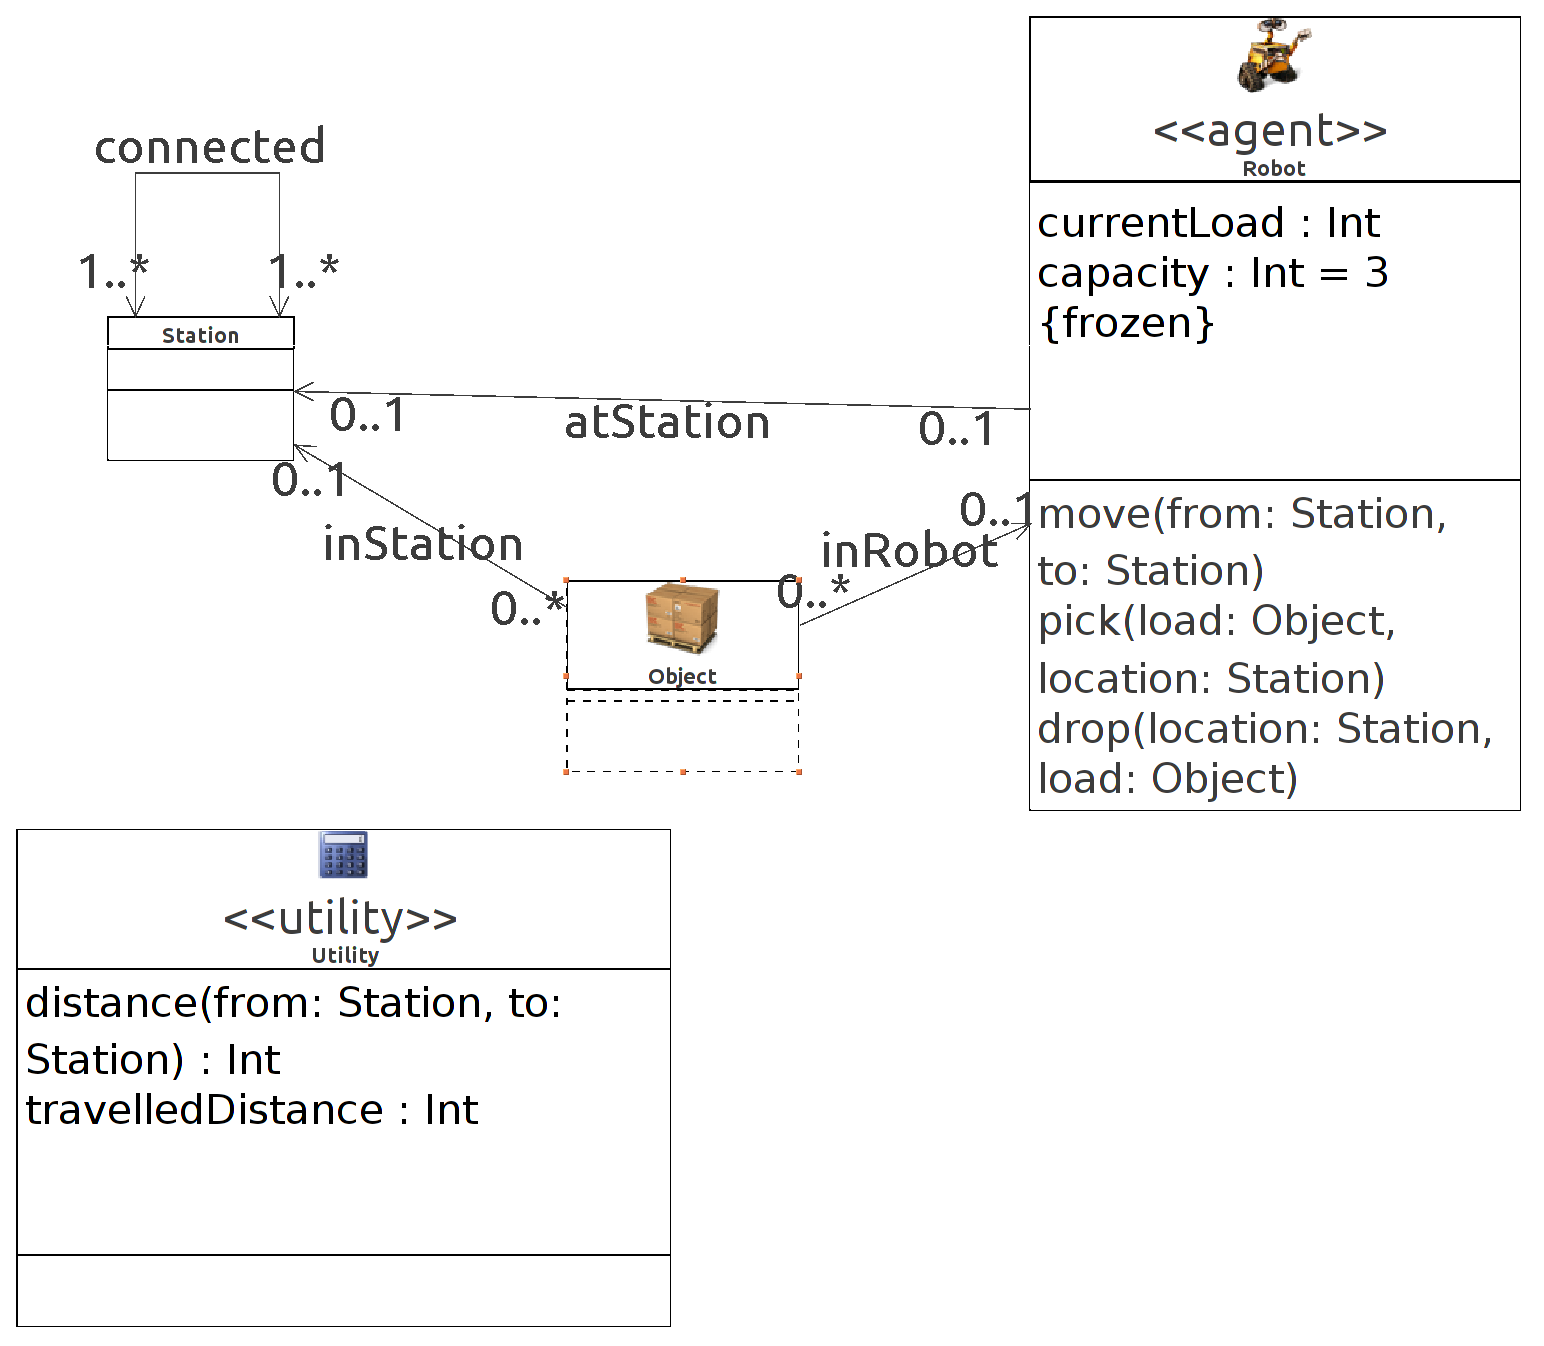
\includegraphics[width=12 cm]{figures/class_diagram.png} 
	\caption{Robocup at work domain: Final class diagram}
	\label{fig:class}
\end{figure}

Problems are defined by instantiating the class diagram with all possible objects and then creating snap shots of the initial state and the goal state. Figure \ref{fig:initial} below shows the initial state for problem 1 while figure \ref{fig:goal} shows its goal state.

\begin{figure}[H] %  figure placement: here, top, bottom, or page
	\centering
	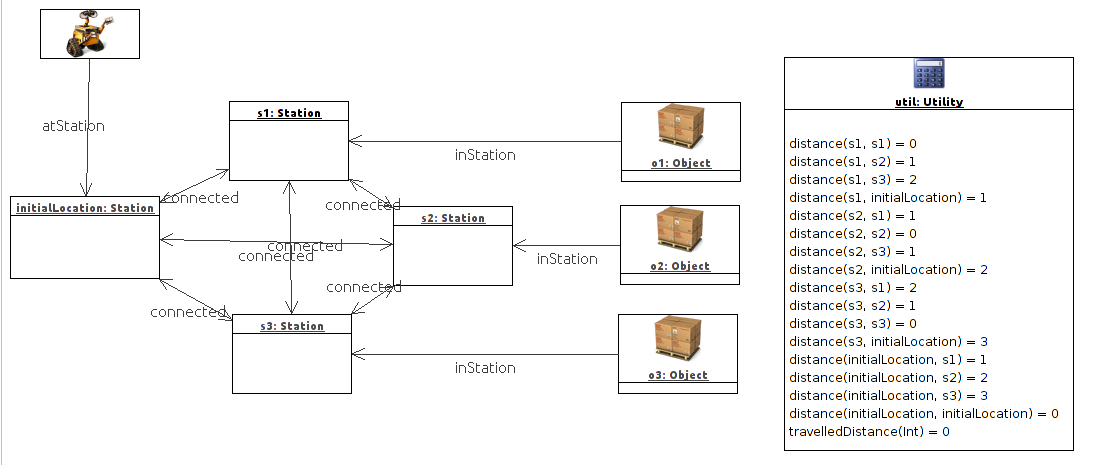
\includegraphics[width=15 cm]{figures/p01_initial_state.png} 
	\caption{Robocup at work domain: P01 Initial state}
	\label{fig:initial}
\end{figure}

\begin{figure}[H] %  figure placement: here, top, bottom, or page
	\centering
	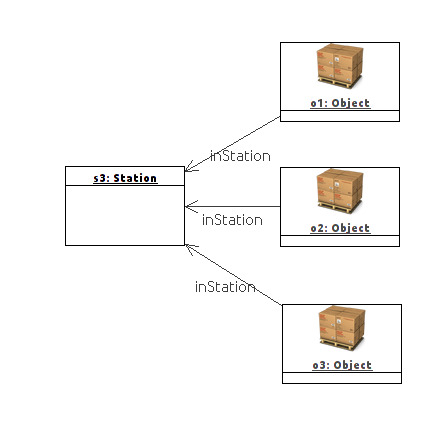
\includegraphics[width=8 cm]{figures/p01_goal.png} 
	\caption{Robocup at work domain: P01 Goal state}
	\label{fig:goal}
\end{figure}

The models of domains and problems are then translated to PDDL. All PDDL files can be found in the files attached to this report.

\newpage
\section{Results}
A summary sheet of the results is as shown in Figure: \ref{fig:Results}. 

\begin{figure}[H] %  figure placement: here, top, bottom, or page
	\centering
	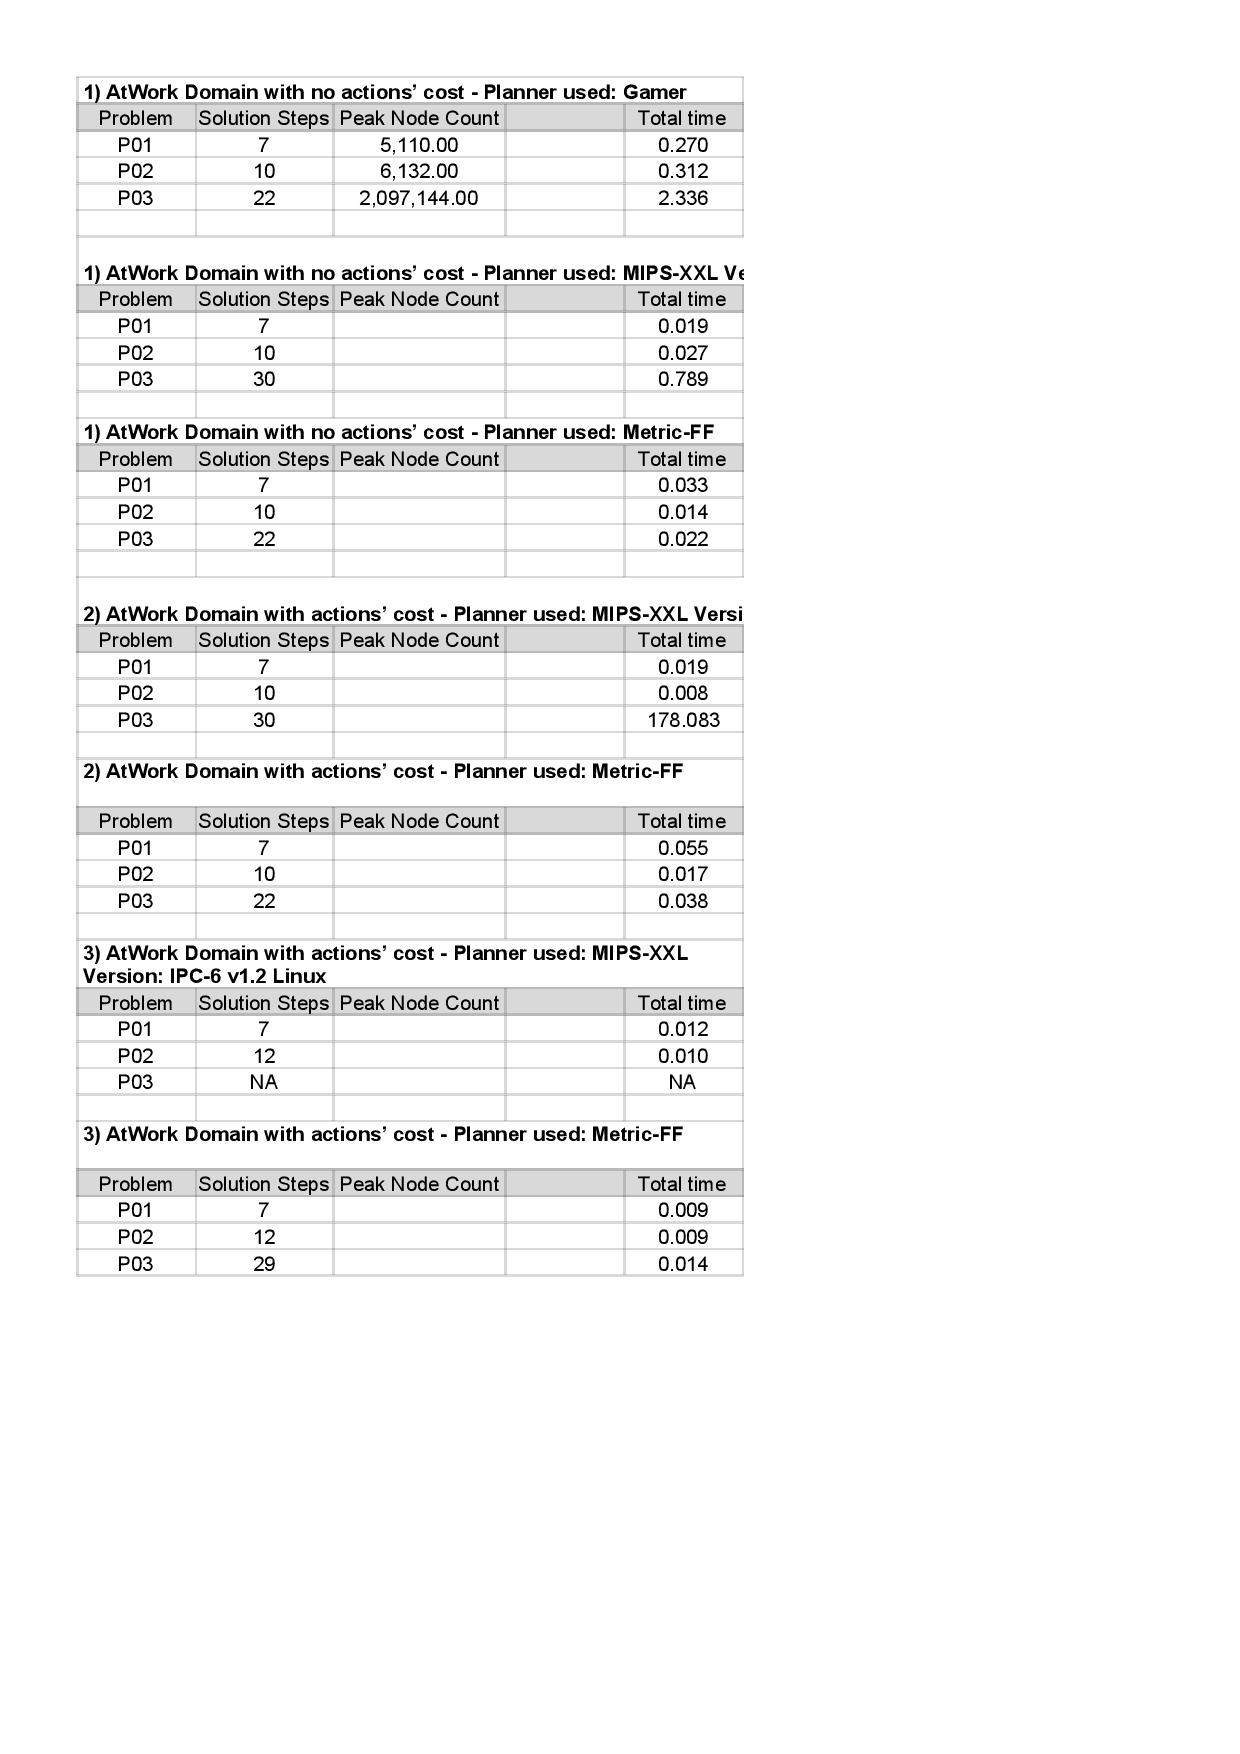
\includegraphics[scale=0.6]{figures/Results_Summary-page-001.jpg} 
	\caption{Result Summary}
	\label{fig:Results}
\end{figure}

Metric\_FF was found to be the fastest and most stable planner in (cGamer, MIPS and METRIC\_FF). cGamer was not able to run the extended domain and raised a parser exception. MIPS could not find a plan for the third P03 with distances and capacity constraints Metric\_FF planned successfully for all the problem and all domains.

\newpage

\bibliography{bib}

\end{document}
